\documentclass[12pt]{scrartcl}

\usepackage{float}

\usepackage[utf8]{inputenc}

\usepackage[T1]{fontenc}

\usepackage{lmodern}

\usepackage[ngerman]{babel}

\usepackage{amsmath}

\usepackage{graphicx}


 

\title{Versuch WO3\\ Beugung und Interferenz von Lichtwellen}

\author{Frederik Strothmann, Henrik Jürgens}

\date{\today}


\begin{document}


 %deckblatt erstellen

\maketitle
\newpage
\tableofcontents
\newpage

%einleitung zu dem experiment

\section{Einleitung}

In der Versuchsreihe WO3 soll die Beugung (Diffraktion) von kohärenten Lichtwellen (Laserlicht) an verschiedenen Öffnungen untersucht werden.
Die Erscheinungen von Beugung und Interferenz sind grundlegend für die Wirkungsweise wichtiger optischer Instrumente. So bestimmt z.B. die Beugung an in der Regel kreisförmigen Öffnungen (z.B. Linsenfassungen) das räumliche Auflösungsvermögen aller optischer Instrumente vom Mikroskop über das menschliche Auge bis hin zu den großen Radioteleskopen. Wir werden zunächst die Intensitätsverteilung des Beugungsmusters eines Einzelspaltes ausmessen und unsere Messungen mit den entsprechenden Rechnungen, die auf dem Huygensschen Prinzip beruhen, vergleichen. Das gleiche werden wir dann anschließend mit den Beugungsbildern einer Lochblende, eines Doppelspaltes und eines Strichgitters durchführen.
%versuchsaufbau mit skizze

\section{Versuchsaufbau}
Der Versuchsaufbau besteht aus einer mikrooptischen Bank, auf der links der Laser und rechts das Intensitätsmessgerät angebracht sind. Zwischen Laser und dem Messgerät ist eine Halterung für die Spalte.

\begin{figure}[H]
\centering
    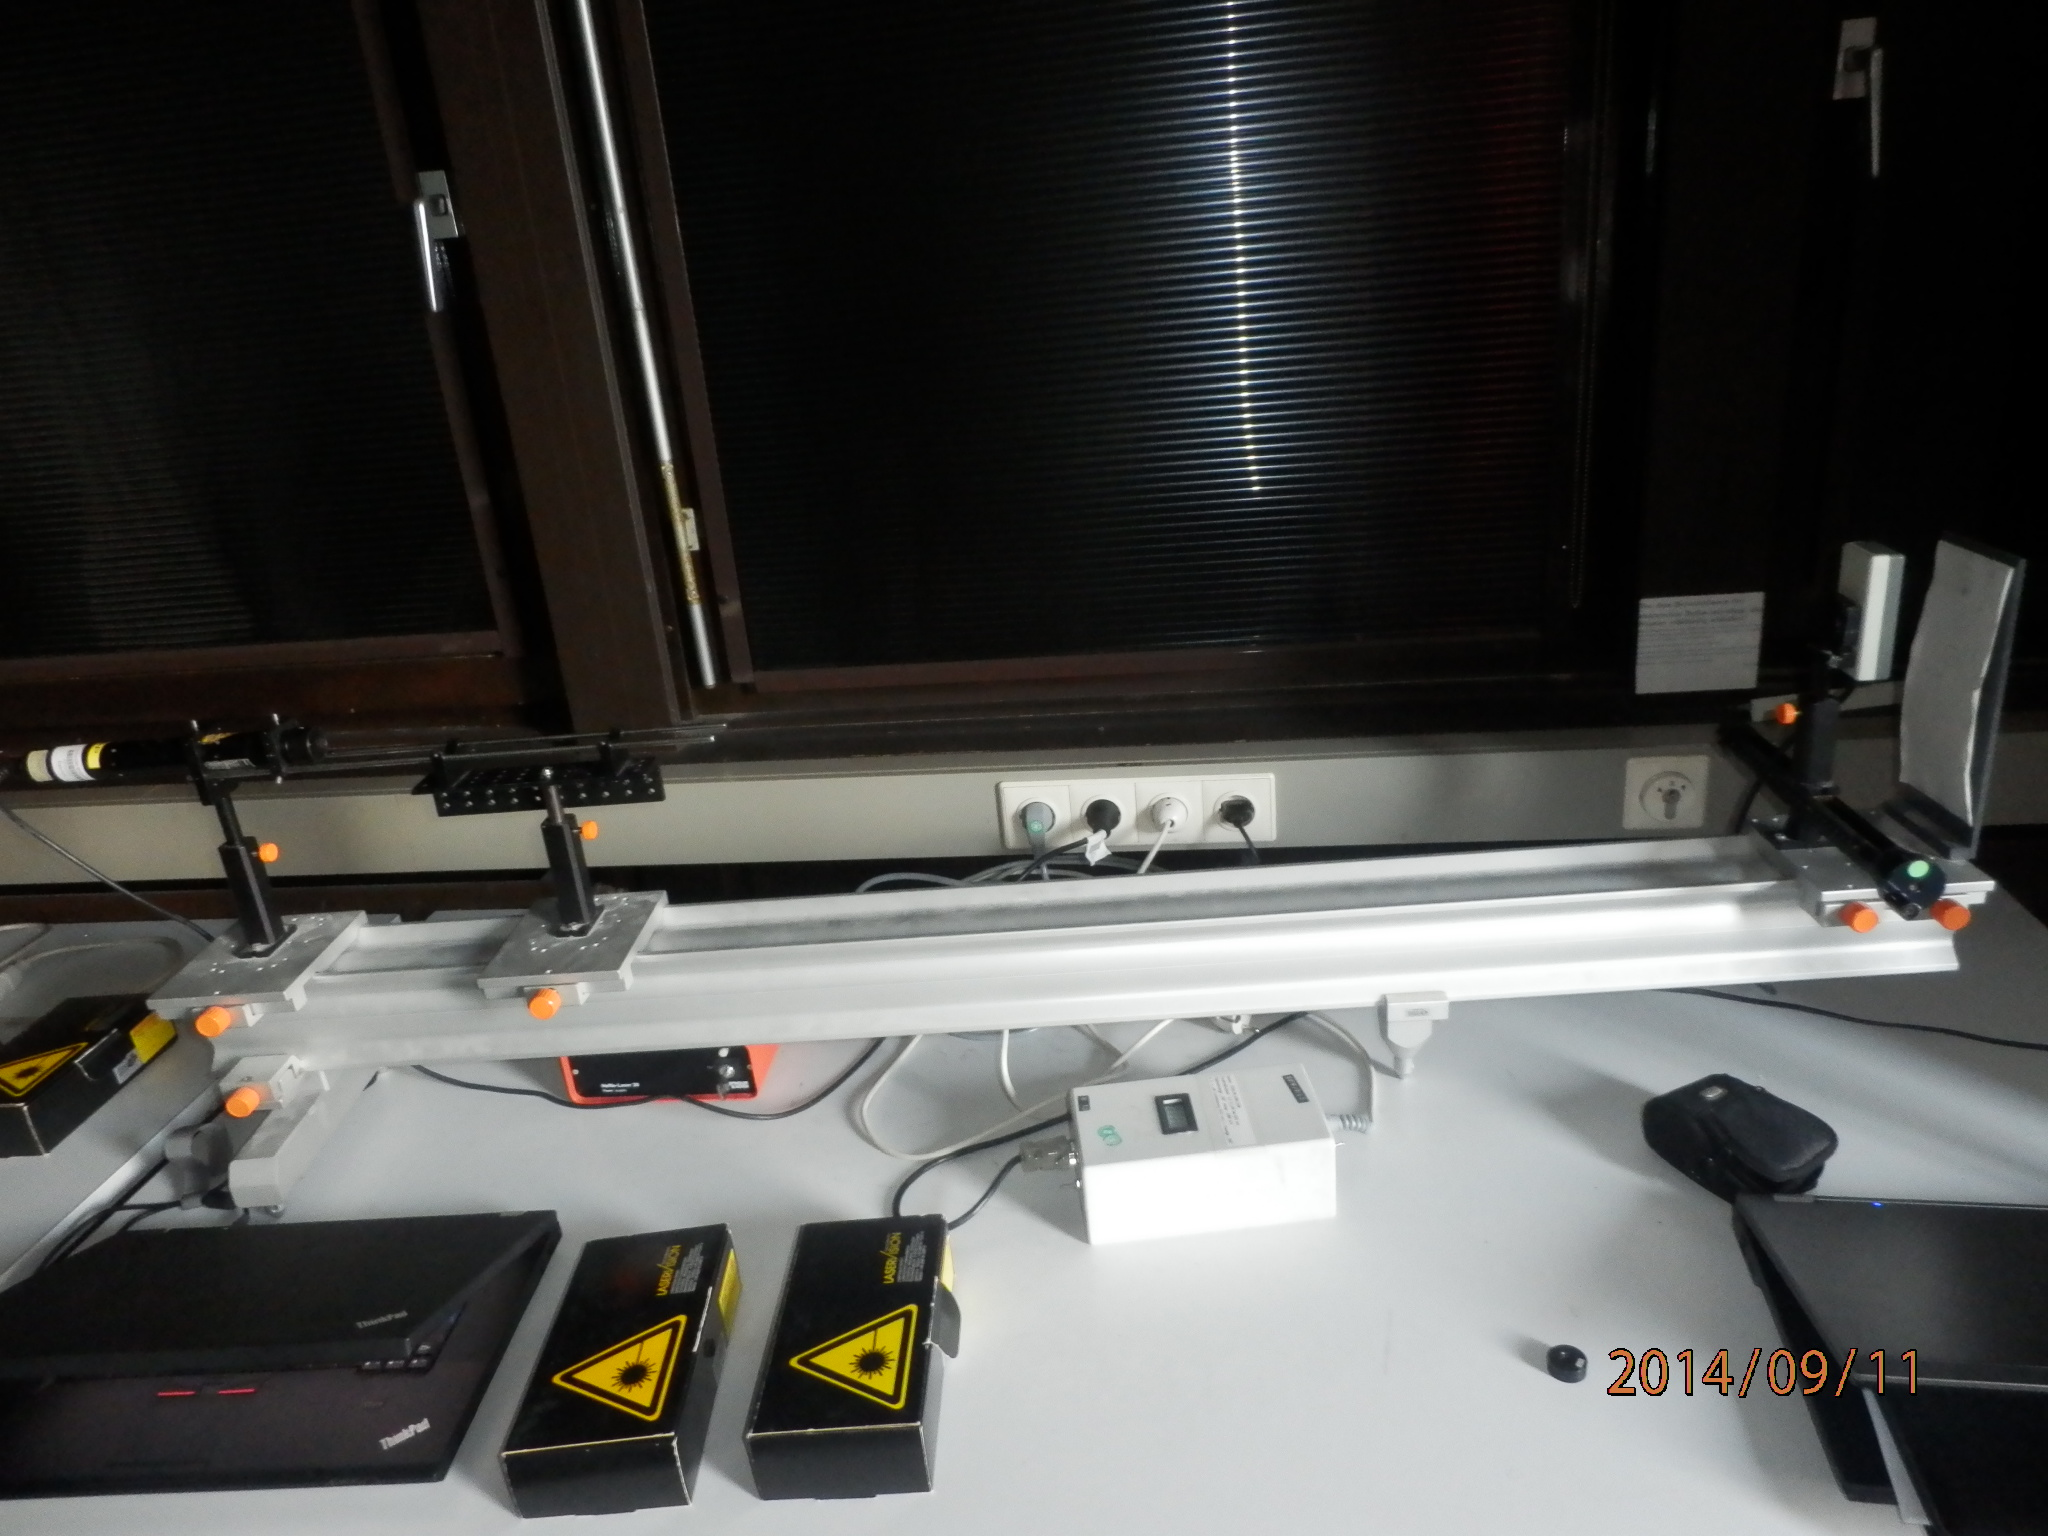
\includegraphics[scale = 0.1]{versuchsaufbau.JPG}
  	\caption[Foto des Versuchsaufbaus]{Foto des Versuchsaufbaus}
  \label{fig:versuchsaufbau}
\end{figure}

\section{Versuch WO3.1: Beugungsmuster eines Einfachspaltes}
\subsection{Versuchsdurchführung}

\subsubsection{Praktische Durchführung}
Wir bauen den in Abbildung 
%\ref{} Abbilung 17 aus der versuchsbeschreibung oder besser eine eigene zeichnung
\begin{figure}[H] 
  \centering
    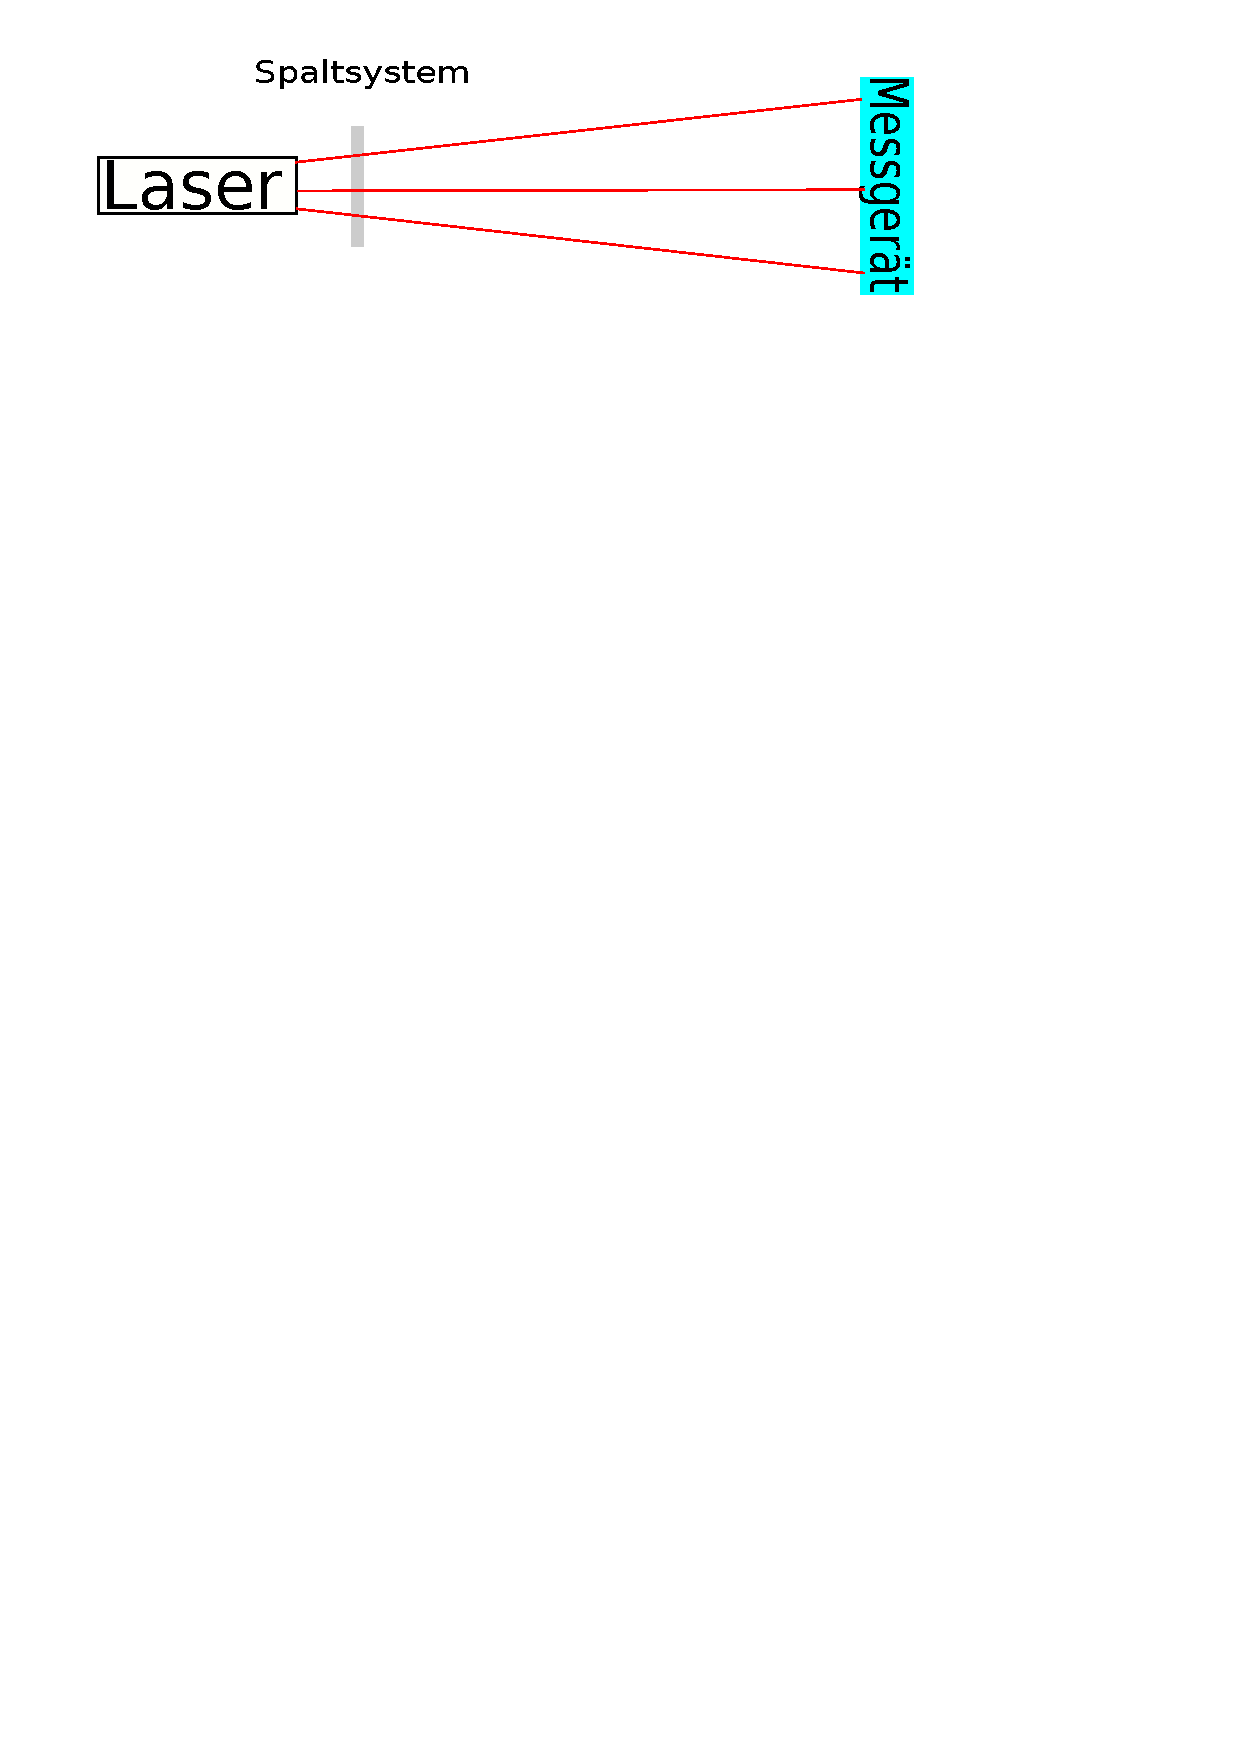
\includegraphics[trim = 0mm 240mm 0mm 10mm, clip, scale = 1]{abb_17.pdf}
  	\caption[Skizze des Aufbaus, auf der optische Bank]{Skizze des Aufbaus, auf der optische Bank\footnotemark}
  \label{fig:abb_17}
\end{figure}

skizzierten Versuchsaufbau mit Elementen der mikrooptischen Bank auf. Als Quelle für kohärente und ebene Wellen verwenden wir einen Neon-Helium-Gaslaser. Die Wellenlänge des Lichtes beträgt $\lambda$ = 0,6328 $\mu$m.
Wir messen die Intensitätsverteilung des Beugungsmusters in der Ebene des "Schirms" mit einem Intensitätsmessggerät aus. Wir tragen dann $\frac{I_\theta}{I_0}$ graphisch auf und vergleichen die Messwerte mit der theoretischen Verteilung. Aus der Lage der ersten Minima bestimmen wir die Wellenlänge $\lambda$.
\subsubsection{Theoretische Durchführung}
Den Winkel $\theta$ berechnen wir im folgenden \textbf{immer} mit der Formel:
\begin{align}
\theta = tan^{-1}(\frac{x}{L})
\end{align}
wobei x der Abstand zum Hauptmaximum und L der Abstand des Gitters zum Intensitätsmessgerät ist.\\
Der Fehler berechnet sich nach folgender Formel:
\begin{align}
\sigma_\theta = \sqrt{
\left(\frac{1}{L\left(1+\left(\frac{x}{L}\right)^2\right)}\sigma_x\right)^2+
\left(\frac{x}{L^2\left(1+\left(\frac{x}{L}\right)^2\right)}\sigma_L\right)^2}
\end{align}

Für die Intensitätsverteilung $I_\theta$ Abhängig vom Winkel $\theta$ erwarten wir folgenden Zusammenhang:
\begin{align}
I_\theta = I_0 \left(\frac{\sin \left(\frac{\pi b \sin{\theta}}{\lambda}\right)}{\frac{\pi b \sin{\theta}}{\lambda}}\right)^2
\label{eqn:I_theta_Einzelspalt}
\end{align}
$I_0$ ist die Intensität bei einer Auslekung von 0$^{\circ}$, $b$ die Breite des Spaltes und $\lambda$ die Wellenlänge des Lasers.

Die Wellenlänge $\lambda$ kann aus der Lage des ersten Minimums bestimmt werden
\begin{align}
\lambda = \sin(\theta) b
\label{eqn:lambda_a_1}
\end{align}
$b$ ist dabei die Breite des Spaltes.\\
Der Fehler für die Wellenlänge ist:
\begin{align}
\sigma_\lambda = \sqrt{
\left(\cos(\theta)b \sigma_\theta\right)^2+
\left(\sin(\theta) \sigma_b\right)^2}
\label{eqn:lambda_a_1_sigma}
\end{align}
\subsection{Messergebnisse}

\begin{table}[H]
\caption{Materialeingschaften der Geräte aus der Messung zum Einzelspalt}
\begin{center}
\begin{tabular}{|l|l|l|l|l|l|}
\hline
Offset/mV & Fehler/mV & Spaltbreite/mm & Fehler/mm & Abstand/mm & Fehler/mm \\ \hline
\multicolumn{1}{|r|}{-1,3} & \multicolumn{1}{r|}{0,1} & \multicolumn{1}{r|}{0,20} & \multicolumn{1}{r|}{0,05} & \multicolumn{1}{r|}{1260} & \multicolumn{1}{r|}{2} \\ \hline
\end{tabular}
\end{center}
\label{tab:a_1_e}
\end{table}

\begin{table}[H]
\caption{Messwerte, der Vermessung des Einzelspaltes}
\begin{center}
\begin{tabular}{|r|r|r|r|}
\hline
\multicolumn{1}{|l|}{Auslenkung/Grad} & \multicolumn{1}{l|}{Fehler/Grad} & \multicolumn{1}{l|}{Intensitätsverhältnis} & \multicolumn{1}{l|}{Fehler} \\ \hline
-0,59 & 0,02 & 0,011516 & 1E-006 \\ \hline
-0,55 & 0,02 & 0,013448 & 2E-006 \\ \hline
-0,50 & 0,02 & 0,00960 & 0,00002 \\ \hline
-0,45 & 0,02 & 0,015355 & 2E-006 \\ \hline
-0,41 & 0,02 & 0,030710 & 2E-006 \\ \hline
-0,36 & 0,02 & 0,028791 & 2E-006 \\ \hline
-0,32 & 0,02 & 0,005758 & 2E-006 \\ \hline
-0,27 & 0,02 & 0,013435 & 2E-006 \\ \hline
-0,23 & 0,02 & 0,047984 & 2E-006 \\ \hline
-0,18 & 0,02 & 0,051823 & 2E-006 \\ \hline
-0,14 & 0,02 & 0,026874 & 2E-006 \\ \hline
-0,09 & 0,02 & 0,14402 & 2E-006 \\ \hline
-0,05 & 0,02 & 0,5489 & 1E-005 \\ \hline
0,00 & 0,02 & 1,00000 & 1E-005 \\ \hline
0,05 & 0,02 & 0,86563 & 2E-005 \\ \hline
0,09 & 0,02 & 0,75435 & 1E-005 \\ \hline
0,12 & 0,02 & 0,45112 & 1E-005 \\ \hline
0,18 & 0,02 & 0,261031 & 3E-006 \\ \hline
0,22 & 0,02 & 0,209225 & 3E-006 \\ \hline
0,27 & 0,02 & 0,140125 & 2E-006 \\ \hline
0,32 & 0,02 & 0,038462 & 2E-006 \\ \hline
0,36 & 0,02 & 0,013426 & 2E-006 \\ \hline
0,41 & 0,02 & 0,026927 & 2E-006 \\ \hline
0,45 & 0,02 & 0,030715 & 2E-006 \\ \hline
0,50 & 0,02 & 0,013421 & 2E-006 \\ \hline
0,55 & 0,02 & 0,00965 & 0,00002 \\ \hline
0,59 & 0,02 & 0,00964 & 0,00002 \\ \hline
\end{tabular}
\end{center}
\label{tab:a_1_m}
\end{table}



\subsection{Auswertung}
Nach Gleichung \ref{eqn:lambda_a_1} sollte die Wellenlänge des Lasers bestimmt werden, der Fehler wurde mit Gleichung \ref{eqn:lambda_a_1_sigma} berechnet. Dabei ergab sich ein Wert von 0,52 $(\pm 0,08) \mu$m. Graphisch ergab sich der folgende Plot (Werte aus Tabelle \ref{tab:a_1_e}).

\begin{figure}[H]
\centering
    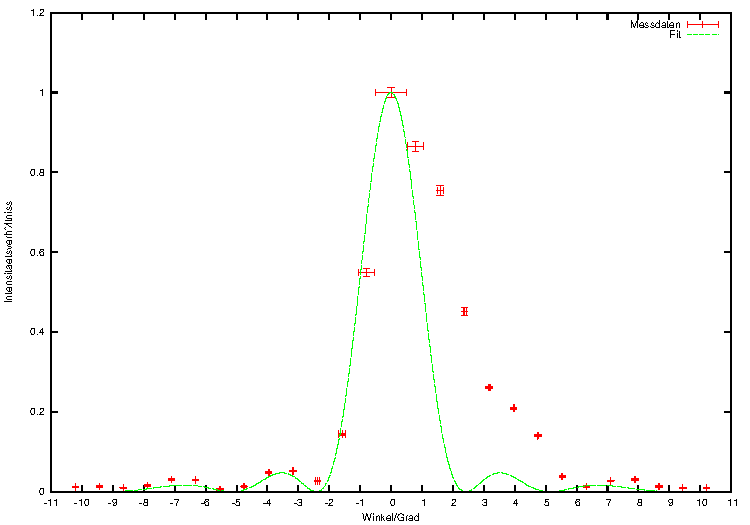
\includegraphics[scale = 1]{a_1.pdf}
  	\caption[Plot des Intensitätsverhältnisses in Abhängigkeit des Winkels, mit theoretischer Vorhersage]{Plot des Intensitätsverhältnisses in Abhängigkeit des Winkels, mit theoretischer Vorhersage}
  \label{fig:a_1}
\end{figure}

\subsection{Diskussion}
Die bestimmte Wellenlänge liegt im $\sigma_2$ Intervall des erwarteten Wertes von 0,63$\mu$m. Die Abweichung kann daraus entstanden sein, dass der Spalt nicht exakt parallel zur Messapparatur eingestellt war.
Die Messwerte liegen auf der linken Seite nah an der Theoriekurve, auf der rechten Seite weichen sie dagegen stark ab, sodass wir nur das linke Minimum zur Berechnung der Wellenlänge verwenden konnten. Die Abweichung zeigt sich auch in späteren Versuchsteilen. Es ist anzunehmen, dass die Lochblende des Lasers auf der rechten Seite beschädigt ist, wodurch die Strahlen eine Streuung zur rechten Seite aufwiesen und dort eine stärkere Intensität zu messen war.
Die Theoriekurven wurden nach Formel \ref{eqn:I_theta_Doppelspalt} bestimmt und mit der angegebenen sowie der aus den Messwerten bestimmten Wellenlänge in den Plot der Daten eingefügt. Es ist unschwer zu erkennen, dass die über die gemessene Wellenlänge bestimmte Kurve besser zu unseren Messwerten passt, wobei der rechte Teil des Plots wie bereits erwähnt nicht zu beachten ist, da offensichtlich  systematische Fehler Einfluss auf unsere Messergebnisse hatten.


\section{Versuch WO3.2: Beugungsmuster einer Kreisblende}
\subsection{Versuchsdurchführung}

\subsubsection{Praktische Durchführung}
Wir verwenden den gleichen Aufbau wie bei Versuch WO3.1. Für diesen Versuch bestimmen wir aus dem Durchmesser der Kreislinie des ersten Minimums den Durchmesser der Lochblende und vergleichen unser Ergebnis mit dem auf der Lochblende angegebenen Wert. Wir bestimmen danach die Winkeldivergenz des Lichtbündels unseres Lasers.
\subsubsection{Theoretische Durchführung}
Der Durchmesser $D$ der Lochblende ist:
\begin{align}
D = \frac{3,8317 \lambda}{\sin(\theta)\pi}
\label{eqn:D}
\end{align}
$\lambda$ ist die Wellenlänge und $\theta$ der Winkel bis zum ersten Minimum. Der Vorfaktor 3,8317 kommt aus der Besselfunktion $I_1$.\\
Der zugehörige Fehler ist:
\begin{align}
\sigma_D = \sqrt{
\left(\frac{3,8317}{\sin(\theta)\pi}\sigma_\lambda \right)^2+
\left(\frac{3,8317\lambda}{\sin^2(\theta)\pi}\cos(\theta)
\sigma_\theta \right)^2}
\label{eqn:D_sigma}
\end{align}

Die Winkeldivergenz $\xi$ berechnet sich durch die Formel:
\begin{align}
\xi = \tan^{-1}\left(\frac{\frac{X-x}{2}}{\Delta L}\right)
\label{eqn:winkeldivergenz}
\end{align}
$\Delta L$ ist der Abstand der beiden Messorte voneinander, X der Durchmesser des weiter entfernten Punktes und x der Durchmesser des näher am Laser liegenden Punktes.
$\xi$ gibt den Öffnungswinkel relativ zur Ausbreitungsrichtung an.

\subsection{Messergebnisse}

\begin{table}[H]
\caption{Materialeigenschaften bei der Lochblende}
\begin{center}
\begin{tabular}{|l|l|l|l|l|l|}
\hline
Offset/mV & Fehler/mV & Durchmesser/mm & Fehler/mm & Abstand/mm & Fehler/mm \\ \hline
\multicolumn{1}{|r|}{-1,3} & \multicolumn{1}{|r|}{0,1} & \multicolumn{1}{r|}{0,25} & \multicolumn{1}{r|}{0,05} & \multicolumn{1}{r|}{1260} & \multicolumn{1}{r|}{0,02} \\ \hline
\end{tabular}
\end{center}
\label{tab:a_2_e}
\end{table}

\begin{table}[H]
\caption{Messwerte, der Vermessung der Lochblende}
\begin{center}
\begin{tabular}{|r|r|r|r|}
\hline
\multicolumn{1}{|l|}{Auslenkung/Grad} & \multicolumn{1}{l|}{Fehler/Grad} & \multicolumn{1}{l|}{Intensitätsverhältniss} & \multicolumn{1}{l|}{Fehler} \\ \hline
-0,59 & 0,02 & 0,003 & 0,001 \\ \hline
-0,55 & 0,02 & 0,003 & 0,001 \\ \hline
-0,50 & 0,02 & 0,003 & 0,001 \\ \hline
-0,45 & 0,02 & 0,003 & 0,001 \\ \hline
-0,41 & 0,02 & 0,003 & 0,001 \\ \hline
-0,36 & 0,02 & 0,022 & 0,001 \\ \hline
-0,32 & 0,02 & 0,042 & 0,001 \\ \hline
-0,27 & 0,02 & 0,032 & 0,001 \\ \hline
-0,23 & 0,02 & 0,032 & 0,001 \\ \hline
-0,18 & 0,02 & 0,013 & 0,001 \\ \hline
-0,14 & 0,02 & 0,109 & 0,001 \\ \hline
-0,09 & 0,02 & 0,380 & 0,002 \\ \hline
-0,05 & 0,02 & 0,768 & 0,006 \\ \hline
0,00 & 0,02 & 1,000 & 0,007 \\ \hline
0,045 & 0,02 & 0,932 & 0,007 \\ \hline
0,09 & 0,02 & 0,642 & 0,006 \\ \hline
0,14 & 0,02 & 0,245 & 0,005 \\ \hline
0,18 & 0,02 & 0,051 & 0,001 \\ \hline
0,23 & 0,02 & 0,013 & 0,001 \\ \hline
0,27 & 0,02 & 0,032 & 0,001 \\ \hline
0,32 & 0,02 & 0,013 & 0,001 \\ \hline
0,36 & 0,02 & -0,007 & 0,001 \\ \hline
0,41 & 0,02 & 0,003 & 0,001 \\ \hline
0,45 & 0,02 & 0,013 & 0,001 \\ \hline
0,50 & 0,02 & 0,0126 & 0,001 \\ \hline
0,55 & 0,02 & 0,003 & 0,001 \\ \hline
0,59 & 0,02 & -0,007 & 0,001 \\ \hline
\end{tabular}
\end{center}
\label{tab:a_2_m}
\end{table}

\begin{table}[H]
\caption{Messdaten zur bestimmung der Winkeldivergenz}
\begin{center}
\begin{tabular}{|l|l|}
\hline
Ausgang/mm & Fehler/mm \\ \hline
\multicolumn{1}{|r|}{2} & \multicolumn{1}{r|}{2} \\ \hline
Weitung/mm & Fehler/mm \\ \hline
\multicolumn{1}{|r|}{12} & \multicolumn{1}{r|}{2} \\ \hline
Abstand/mm & Fehler/mm \\ \hline
\multicolumn{1}{|r|}{6100} & \multicolumn{1}{r|}{20} \\ \hline
\end{tabular}
\end{center}
\label{tab:a_2_w}
\end{table}


\subsection{Auswertung}
Es sollte der Durchmesser der Lochblende bestimmt werden, dafür wurde der Abstand zwischen den ersten beiden Minima verwendet und halbiert. Zur Berechnung des Durchmessers wurde Gleichung \ref{eqn:D} und Gleichung \ref{eqn:D_sigma} für den Fehler verwendet. Dabei ergab sich ein Wert von 0,30 $(\pm 0,05)$mm. Graphisch ergibt sich eine durch das Intensitätsmaximum $I_0$ normierte Intensitätsverteilung (Werte aus Tabelle \ref{tab:a_2_m}).

\begin{figure}[H]
\centering
    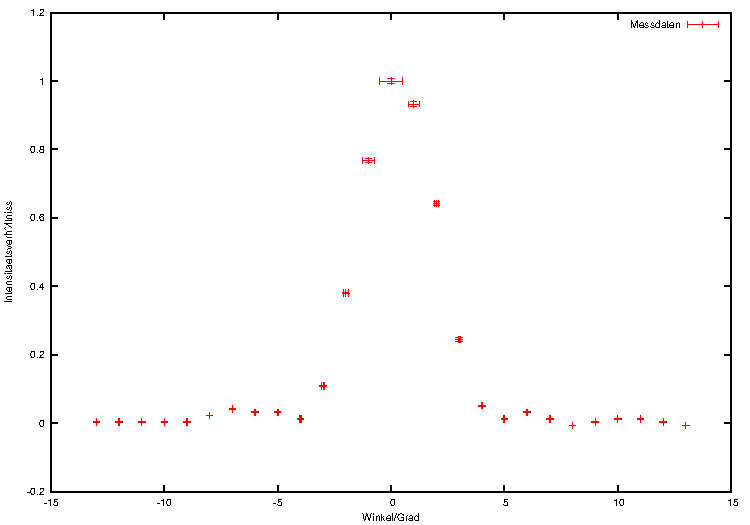
\includegraphics[scale = 1]{a_2.pdf}
  	\caption[Plot des Intensitätsverhältnisses in Abhängigkeit des Winkels, mit smooth csplines (Punkte verbinden)]{Plot des Intensitätsverhältnisses in Abhängigkeit des Winkels, mit smooth csplines (Punkte verbinden)}
  \label{fig:a_2}
\end{figure}

%es fehlt noch die auswertung der Winkeldivergenz. was du machen musst habe ich in den Theorieteil eingefügt. in die diskussion hab ich auch schon einen Satz geschrieben.
Für die  Bestimmung der  der Winkeldivergenz wurde Gleichung \ref{eqn:winkeldivergenz}, es ergab sich eine Winkeldivergenz von 0,05 Grad.

\subsection{Diskussion}
Auf der Lochblende war ein Durchmesser von 0,2 mm angegeben. Dieser Wert liegt erst im $\sigma_3$ Intervall des gemessenen Wertes, welcher nach Formel \ref{eqn:D} berechnet wurde. Diese Abweichung begründet sich dadurch, dass das Intensitätsmessgerät zum einen leicht um die
Längsachse verdreht war, sodass zusätzliche Messungenauigkeiten entstanden sind, und zum anderen durch den Defekt der Lochblende des Lasers, welcher auch bei dieser Messung an der Intensitätsverteilung des Hauptmaximums zu beobachten war. Neben diesen Fehlern war bei dem Versuch auch die Streuung des Laserlichtes deutlich zu erkennen.
Die Winkeldivergenz haben wir an dem Laser der Nachbargruppe ausgemessen, da dieses bereits aus der Halterung gelöst war und wir zu wenig Zeit für eine Eigene Messung hatten. Da wir für unseren Eigenen Laser nicht die Winkeldivergenz bestimmen konnten, ist nicht bekannt, ob die Lochblende des Lasers defekt war oder nicht.

\section{Versuch WO3.3: Beugungsmuster eines Doppelspaltes}
\subsection{Versuchsdurchführung}

\subsubsection{Praktische Durchführung}
Wir messen die Intensität des Doppelspaltes aus und stellen unsere Messergebnisse graphisch dar, sowie vergleichen sie mit der theoretischen Vorhersage. Wir berechnen danach die Wellenlänge.
\subsubsection{Theoretische Durchführung}
Die Wellenlänge $\lambda$ berechnet sich durch:
\begin{align}
\lambda = \frac{2d \sin(\theta)}{2n-1}
\label{eqn:lambda_2}
\end{align}
$n$ ist die Ordung des Minimums, d der Abstand des Doppelspaltes.
Der Fehler ergibt sich durch:
\begin{align}
\sigma_\lambda = \sqrt{
\left(\frac{2 \sin(\theta)}{2n-1}\sigma_d\right)^2+
\left(\frac{2d \cos(\theta)}{2n-1}\sigma_\theta\right)^2}
\label{eqn:lambda_2_sigma}
\end{align}
Für die Intensitätsverteilung $I_\theta$ erwarten wir folgenden Zusammenhang:
\begin{align}
I_\theta = I_0\left(\frac{\sin\left(\frac{\pi b \sin(\theta)}{\lambda}\right)}{\frac{\pi b \sin(\theta)}{\lambda}}\cos\left(\frac{\pi d\sin(\theta)}{\lambda}\right)\right)^2
\label{eqn:I_theta_Doppelspalt}
\end{align}
$b$ ist dabei die Breite der Spalte, $d$ der Abstand der beiden Spalte und $\lambda$ die Wellenlänge des Lasers.

\subsection{Messergebnisse}

\begin{table}[H]
\caption{Materialeingenschaften, für die Messung des Doppelspaltes}
\begin{center}
\begin{tabular}{|l|l|l|l|}
\hline
Offset/mV & Fehler/mV & Durchmesser/mm & Fehler/mm \\ \hline
\multicolumn{1}{|r|}{-1,3} & \multicolumn{1}{|r|}{0,1} & \multicolumn{1}{r|}{0,25} & \multicolumn{1}{r|}{0,05} \\ \hline
Abstand schlitze/mm & Fehler/mm & Abstand/mm & Fehler/mm \\ \hline
\multicolumn{1}{|r|}{0,75} & \multicolumn{1}{r|}{0,05} & \multicolumn{1}{r|}{1260} & \multicolumn{1}{r|}{20} \\ \hline
\end{tabular}
\end{center}
\label{tab:a_3_e}
\end{table}



\begin{table}[H]
\caption{Messwerte, der Vermessung des Doppelspaltes}
\begin{center}
\begin{tabular}{|r|r|r|r|}
\hline
\multicolumn{1}{|l|}{Auslenkung/Grad} & \multicolumn{1}{l|}{Fehler/Grad} & \multicolumn{1}{l|}{Intensitätsverhältniss} & \multicolumn{1}{l|}{Fehler} \\ \hline
-0,8639 & 0,0001 & 0,011 & 0,002 \\ \hline
-0,8184 & 0,0001 & 0,002 & 0,002 \\ \hline
-0,7729 & 0,0001 & 0,005 & 0,002 \\ \hline
-0,7275 & 0,0001 & 0,017 & 0,002 \\ \hline
-0,6820 & 0,0001 & 0,002 & 0,002 \\ \hline
-0,6365 & 0,0001 & 0,010 & 0,001 \\ \hline
-0,5911 & 0,0001 & 0,024 & 0,002 \\ \hline
-0,5456 & 0,0001 & 0,002 & 0,002 \\ \hline
-0,5001 & 0,0001 & 0,019 & 0,002 \\ \hline
-0,4547 & 0,0001 & 0,041 & 0,002 \\ \hline
-0,4092 & 0,0001 & 0,002 & 0,002 \\ \hline
-0,3637 & 0,0001 & 0,044 & 0,002 \\ \hline
-0,3183 & 0,0001 & 0,085 & 0,002 \\ \hline
-0,2728 & 0,0001 & 0,003 & 0,002 \\ \hline
-0,2273 & 0,0001 & 0,131 & 0,002 \\ \hline
-0,1819 & 0,0002 & 0,243 & 0,002 \\ \hline
-0,1364 & 0,0001 & 0,011 & 0,002 \\ \hline
-0,0909 & 0,0007 & 0,907 & 0,002 \\ \hline
-0,0454 & 0,0007 & 1,000 & 0,001 \\ \hline
0,0000 & 0,0007 & 1,000 & 0,002 \\ \hline
0,0454 & 0,0007 & 1,000 & 0,002 \\ \hline
0,0909 & 0,0005 & 1,000 & 0,001 \\ \hline
0,1364 & 0,0001 & 0,021 & 0,002 \\ \hline
0,1819 & 0,0001 & 0,156 & 0,002 \\ \hline
0,2273 & 0,0001 & 0,122 & 0,002 \\ \hline
0,2728 & 0,0001 & 0,004 & 0,002 \\ \hline
0,3183 & 0,0001 & 0,065 & 0,002 \\ \hline
0,3637 & 0,0001 & 0,038 & 0,002 \\ \hline
0,4092 & 0,0001 & 0,002 & 0,002 \\ \hline
0,4547 & 0,0001 & 0,032 & 0,002 \\ \hline
0,5002 & 0,0001 & 0,016 & 0,002 \\ \hline
0,5456 & 0,0001 & 0,001 & 0,002 \\ \hline
0,5911 & 0,0001 & 0,019 & 0,002 \\ \hline
0,6366 & 0,0001 & 0,010 & 0,002 \\ \hline
0,6820 & 0,0001 & 0,002 & 0,002 \\ \hline
0,7275 & 0,0001 & 0,013 & 0,002 \\ \hline
0,7729 & 0,0001 & 0,005 & 0,002 \\ \hline
0,8185 & 0,0001 & 0,001 & 0,002 \\ \hline
0,8639 & 0,0001 & 0,007 & 0,002 \\ \hline
0,9094 & 0,0001 & 0,002 & 0,002 \\ \hline
0,9548 & 0,0001 & 0,001 & 0,002 \\ \hline
\end{tabular}
\end{center}
\label{tab:a_3_m}
\end{table}


\subsection{Auswertung}
In der dritten Aufgabe sollte der Intensitätsverlauf eines Doppelspaltes gemessen werden und nach Gleichung \ref{eqn:lambda_2} (für den Fehler Gleichung \ref{eqn:lambda_2_sigma}) die Wellenlänge des Lasers bestimmt werden. Es ergab sich ein Wert von 0,069 $(\pm 0,008) \mu$m.
Graphisch ergibt sich der folgende Plot (Werte aus Tabelle \ref{tab:a_3_m}).

\begin{figure}[H]
\centering
    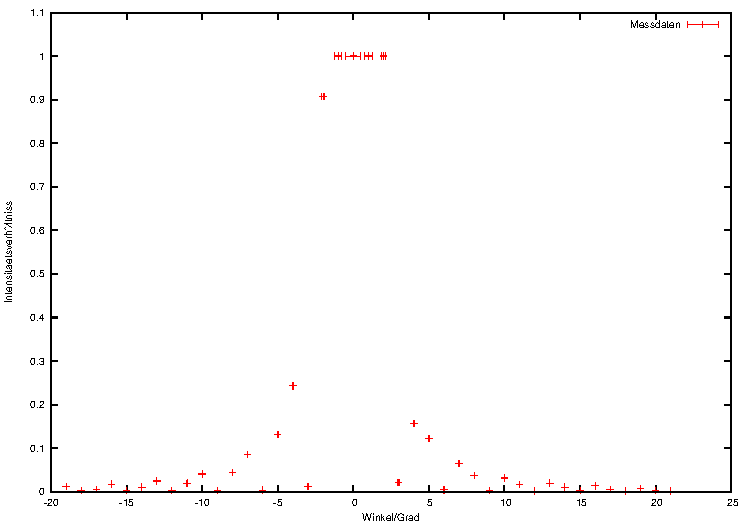
\includegraphics[scale = 1]{a_3.pdf}
  	\caption[Plot des Intensitätsverhältnisses in Abhängigkeit des Winkels, mit theoretischer Vorhersage]{Plot des Intensitätsverhältnisses in Abhängigkeit des Winkels, mit theoretischer Vorhersage}
  \label{fig:a_3}
\end{figure}


\subsection{Diskussion}
Der erwartete Wert für die Wellenlänge war 0,63$\mu$m, dieser liegt innerhalb des $\sigma_1$ Intervalls des gemessenen Wertes 0,069 $(\pm 0,008) \mu$m. Die Theoretische Vorhersage weicht stark von den gemessenen Werten ab, dies betrifft jedoch nur die Amplitude, nicht die Position der Minima und Maxima. Der Fehler kommt daher, dass das Messgerät eine Begrenzung bei 9920 mV hat, was wir einerseits während des Versuches nicht wussten und andererseits mit einem Intensitätsfilter hätte behoben werden können. Durch diesen Fehler ist $\frac{I_\theta}{I_0}$ ,wie man in Abbildung \ref{fig:a_3} gut erkennen kann, viel zu klein geraten. Wir haben zusätzliche theoretische Plots nach Formel \ref{eqn:I_theta_Doppelspalt} mit einem Korrekturfaktor von 4,75 in unsere Messdaten eingefügt, da man so viel besser erkennen kann, dass die theoretische Lage der Maxima und Minima wie bereits erwähnt gut zu den Messergebnissen passt. Dies haben wir für die angegebe, als auch für die aus den Messergebnissen berechnete Wellenlänge gemacht, wobei sich herausstellte, dass die gemessene Wellenlänge wie in Aufgabe 1 besser zu unseren Daten passte.

\section{Versuch WO3.4: Beugungsmuster eines Gitters}
\subsection{Versuchsdurchführung}

\subsubsection{Praktische Durchführung}
Bei dem in diesem Versuchsteil verwendeten Gitter liegt die Gitterkonstante im Bereich von ca. 10$^{-2}$cm. Wir bestimmen aus der Intensitätsverteilung und der Gitterkonstante $d$ die Wellenlänge des Laserlichtes.
\subsubsection{Theoretische Durchführung}
Die Wellenlänge $\lambda$ bestimmen wir durch die Formel:
\begin{align}
\lambda = \frac{\sin(\theta) d}{n}
\label{eqn:lambda_3}
\end{align}
$d$ ist die Gitterkonstante, $n$ die Ordnung des Maximums und $\theta$ die Winkeldifferenz zwischen Hauptmaximum und Nebenmaximum.
Der Fehler berechnet sich durch:
\begin{align}
\sigma_\lambda = \sqrt{
\left(\frac{\cos(\theta) d}{n}\sigma_\theta\right)^2+
\left(\frac{\sin(\theta)}{n}\sigma_d\right)^2}
\label{eqn:lambda_3_sigma}
\end{align}
Für die Intensitätsverteilung $I_\theta$ erwarten wir folgenden Zusammenhang:
\begin{align}
I_\theta = I_0\left(\frac{\sin\left(\frac{\pi d \sin(\theta)}{2\lambda}\right)}{\frac{\pi d \sin(\theta)}{2\lambda}}
\frac{\sin\left(\frac{N \pi d \sin(\theta)}{\lambda}\right)}{\sin\left(\frac{\pi d \sin(\theta)}{\lambda}\right)}\right)^2
\end{align}
$b$ ist dabei die Breite der Spalte, $d$ der Abstand der beiden Spalte und $\lambda$ die Wellenlänge des Lasers.

\subsection{Messergebnisse}

\begin{table}[H]
\caption{Materialeigenschaften, aus der Messung des Gitters}
\begin{center}
\begin{tabular}{|l|l|l|l|l|l|}
\hline
Offset/mV & Fehler/mV & Gitterkonstante/(1/cm) & Fehler/(1/cm) & Abstand/mm & Fehler/mm \\ \hline
\multicolumn{1}{|r|}{-1,3} & \multicolumn{1}{r|}{0,1} & \multicolumn{1}{r|}{80} & \multicolumn{1}{r|}{2} & \multicolumn{1}{r|}{1260} & \multicolumn{1}{r|}{20} \\ \hline
\end{tabular}
\end{center}
\label{tab:a_4_m}
\end{table}


\begin{table}[H]
\caption{Messwerte der Messung des Gitters (1/2)}
\begin{center}
\begin{tabular}{|r|r|r|r|}
\hline
\multicolumn{1}{|l|}{Auslenkung/Grad} & \multicolumn{1}{l|}{Fehler/Grad} & \multicolumn{1}{l|}{Intensitätsverhältnis} & \multicolumn{1}{l|}{Fehler} \\ \hline
-1,14 & 0,02 & 0,0003 & 0,0001 \\ \hline
-1,09 & 0,02 & 0,0003 & 0,0001 \\ \hline
-1,05 & 0,02 & 0,0013 & 0,0001 \\ \hline
-1,00 & 0,01 & 0,0214 & 0,0001 \\ \hline
-0,95 & 0,02 & 0,0315 & 0,0001 \\ \hline
-0,91 & 0,02 & 0,0053 & 0,0001 \\ \hline
-0,86 & 0,02 & 0,0033 & 0,0001 \\ \hline
-0,82 & 0,02 & 0,0033 & 0,0001 \\ \hline
-0,77 & 0,02 & 0,0013 & 0,0001 \\ \hline
-0,73 & 0,02 & 0,0073 & 0,0001 \\ \hline
-0,68 & 0,01 & 0,0698 & 0,0001 \\ \hline
-0,65 & 0,02 & 0,2862 & 0,0002 \\ \hline
-0,59 & 0,02 & 0,0728 & 0,0001 \\ \hline
-0,55 & 0,02 & 0,0063 & 0,0001 \\ \hline
-0,50 & 0,02 & 0,0043 & 0,0001 \\ \hline
-0,45 & 0,02 & 0,0023 & 0,0001 \\ \hline
-0,41 & 0,02 & 0,0144 & 0,00018 \\ \hline
-0,36 & 0,02 & 0,2772 & 0,0002 \\ \hline
-0,32 & 0,02 & 1,0000 & 0,0005 \\ \hline
-0,27 & 0,02 & 0,4785 & 0,0003 \\ \hline
-0,23 & 0,02 & 0,0124 & 0,0001 \\ \hline
-0,18 & 0,02 & 0,0073 & 0,0001 \\ \hline
-0,15 & 0,01 & 0,0073 & 0,0005 \\ \hline
-0,09 & 0,02 & 0,0184 & 0,0005 \\ \hline
-0,05 & 0,02 & 0,1725 & 0,0005 \\ \hline
0,00 & 0,02 & 1,0000 & 0,0007 \\ \hline
\end{tabular}
\end{center}
\label{tab:a_4_e_a}
\end{table}



\begin{table}[H]
\caption{Messwerte der Messung des Gitters (2/2)}
\begin{center}
\begin{tabular}{|r|r|r|r|}
\hline
\multicolumn{1}{|l|}{Auslenkung/Grad} & \multicolumn{1}{l|}{Fehler/Grad} & \multicolumn{1}{l|}{Intensitätsverhältnis} & \multicolumn{1}{l|}{Fehler} \\ \hline
0,05 & 0,02 & 0,3496 & 0,0005 \\ \hline
0,09 & 0,02 & 0,0235 & 0,0001 \\ \hline
0,14 & 0,02 & 0,0023 & 0,0001 \\ \hline
0,18 & 0,02 & 0,0084 & 0,0001 \\ \hline
0,23 & 0,02 & 0,0114 & 0,0001 \\ \hline
0,27 & 0,02 & 0,0718 & 0,0001 \\ \hline
0,32 & 0,02 & 0,3688 & 0,0002 \\ \hline
0,36 & 0,02 & 0,1241 & 0,0001 \\ \hline
0,41 & 0,02 & 0,0225 & 0,0001 \\ \hline
0,45 & 0,02 & 0,0013 & 0,0001 \\ \hline
0,50 & 0,02 & 0,0043 & 0,0001 \\ \hline
0,55 & 0,02 & 0,0053 & 0,0001 \\ \hline
0,59 & 0,02 & 0,0114 & 0,0001 \\ \hline
0,64 & 0,02 & 0,0134 & 0,0001 \\ \hline
0,68 & 0,02 & 0,0063 & 0,0001 \\ \hline
0,73 & 0,01 & 0,0043 & 0,0001 \\ \hline
0,77 & 0,02 & 0,0013 & 0,0001 \\ \hline
0,82 & 0,02 & 0,0104 & 0,0001 \\ \hline
0,86 & 0,02 & 0,0003 & 0,0001 \\ \hline
0,91 & 0,02 & 0,0003 & 0,0001 \\ \hline
0,95 & 0,02 & 0,0003 & 0,0001 \\ \hline
\end{tabular}
\end{center}
\label{tab:a_4_e_b}
\end{table}



\subsection{Auswertung}
Aus der Intensitäsmessung des Gitters sollte die Wellenlänge des Laserstrahls bestimmt werden. Dafür wurde Gleichung \ref{eqn:lambda_3} und für den Fehler Gleichung \ref{eqn:lambda_3_sigma} verwendet. Es ergab sich ein Wert von 0,69 $(\pm  0,08)\mu$m. Graphisch ergibt sich der folgende Plot (Werte aus Tabelle \ref{tab:a_4_m}).

\begin{figure}[H]
\centering
    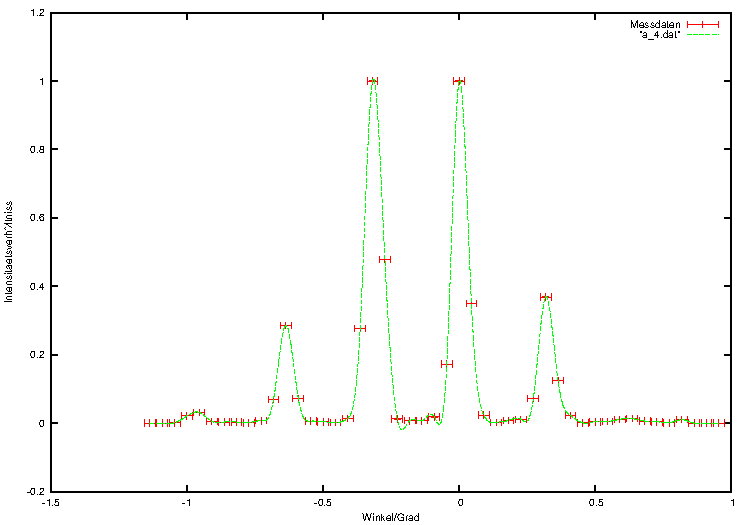
\includegraphics[scale = 1]{a_4.pdf}
  	\caption[Plot des Intensitätsverhältnisses in Abhängigkeit des Winkels, mit smooth csplines (Punkte verbinden)]{Plot des Intensitätsverhältnisses in Abhängigkeit des Winkels, mit smooth csplines (Punkte verbinden)}
  \label{fig:a_4}
\end{figure}


\subsection{Diskussion}
Der im Versuchsprotokoll angegebene Wert für die Wellenlänge des Laserlichts ist mit 0,63$\mu$m angegeben, dieser Wert liegt im $\sigma_1$ Intervall unseres Messwertes. Die Lage des Lasers wurde vor der Messung nochmal justiert, da die Lage des Interferenzmusters zu niedrig war. Es wurde beim Hauptmaximum so wie beim ersten linken Nebenmaximum wie in Aufgabe 3 die Anzeigeskala überschritten. Das erste Nebenmaximum auf der rechten Seite beträgt von der Amplitude nur ein drittel des gemessenen Wertes des anderen ersten Nebenmaximums. Dieser Fehler war reproduzierbar mit dem von uns gewähltem Gitter. Neben dem bekannten Fehler unseres Lasers, dessen Einfluss wir nach der Justierung nicht mehr abschätzen konnten, kann nicht genau bestimmt werden, ob zusätzlich ein Fehler von unserem Gitter ausging, da wir keine Zeit für die Messung mit einem weiteren Gitter hatten.

\section{Fazit}


In Aufgabe 1 gab es bei der Messung des Beugungsmusters des Einfachspaltes Probleme beim Einstellen des Lasers, da auf der rechten Seite kein Interferenzmuster zu erkennen war.
In Abbildung \ref{fig:a_1} kann man diesen deutlichen Fehler gut erkennen, welcher warscheinlich auf eine defekte Lochblende zurückzuführen ist. Ebenso gab es in Aufgabe 4 Probleme bei der Messung der Maxima des Gitterinterferenzmusters, welche vermutlich auf die gleiche Ursache wie in Aufgabe 1 zurückzuführen sind. Der Laser wurde während der Messung gedreht, sodass der so verursachte Fehler das Messergebnis stark beeinträchtigt und der entstandene Fehler nicht aus der ersten Aufgabe abgeleitet werden konnte.
In Aufgabe 3 und 4 haben wir für einige Maxima die gleiche Intensität gemessen, was daran liegt, dass unser Intensitätsmessgerät keine höheren Werte als 9920mV anzeigen konnte. Dies ist uns zu spät aufgefallen und hat zur Folge, dass wir in Aufgabe 3 und 4 einen zu kleinen Wert für $I_0$ gemessen haben.
In Aufgabe 3 ist unsere Abweichung zum Vergleichswert ungewöhnlich groß, was auf verschiedene Ursachen wie z.B. die starke Steuung des Laserlichtes oder das nicht ganz runde Interferenzmuster zurückzuführen ist. Insgesamt sind die Resultate in diesem Versuch eher schlecht ausgefallen, da die Messung mit teilweise defekten Geräten durchgeführt werden musste.

%Werte stimmen mit den Formeln überein/nicht überein

\end{document}

